\documentclass[a4paper]{report}
\usepackage[round]{natbib}

\usepackage{Rnews}
\usepackage{fancyvrb}
\usepackage{Sweave}  

\DefineVerbatimEnvironment{Sinput}{Verbatim}{fontsize=\small,fontshape=sl}
\DefineVerbatimEnvironment{Soutput}{Verbatim}{fontsize=\small}
\DefineVerbatimEnvironment{Scode}{Verbatim}{fontsize=\small,fontshape=sl}

%% \SweaveOpts{prefix.string=graphics/portfolio}

\bibliographystyle{abbrvnat}

\begin{document}
\begin{article}
\title{Backtests}
\author{Kyle Campbell, Jeff Enos, Daniel Gerlanc and David Kane}

%%\VignetteIndexEntry{Using the backtest package}
%%\VignetteDepends{backtest}


\maketitle

\setkeys{Gin}{width=0.95\textwidth}

\section*{Introduction}

The \pkg{backtest} package provides facilities for exploring
portfolio-based hypotheses about financial instruments (stocks, bonds,
swaps, options, et cetera).  For example, consider a claim that stocks
for which analysts are raising their earnings estimates perform better
than stocks for which analysts are lowering estimates.  We want to
examine if, on average, stocks with raised estimates have higher
future returns than stocks with lowered estimates and whether this is
true over various time horizons and across different categories of
stocks.  Colloquially, ``backtest'' is the term used in finance for
such tests.

\section*{Background}

StarMine\footnote{See www.starmine.com for details.} is a San
Fransisco research company which creates quantitative equity models
for stock selection. According to the company:

% Note that we make the font size for this quote small and then go
% back to normal.

\small

\begin{quote}
  StarMine Indicator is a 1-100 percentile ranking of stocks that is
  predictive of future analyst revisions. StarMine Indicator improves
  upon basic earnings revisions models by:

\begin{itemize}
\item Explicitly considering management guidance.
  
\item Incorporating SmartEstimates, StarMine's superior estimates
  constructed by putting more weight on the most accurate analysts.
  
\item Using a longer-term (forward 12-month) forecast horizon (in
  addition to the current quarter).

\end{itemize}

StarMine Indicator is positively correlated to future stock price
movements. Top-decile stocks have annually outperformed bottom-decile
stocks by 27 percentage points over the past ten years across all
global regions.
\end{quote}

\normalsize

These ranks and other attributes of stocks are in the
\texttt{starmine} data frame, available as part of the
\pkg{backtest} package.


\begin{Schunk}
\begin{Sinput}
> data(starmine)
> names(starmine)
\end{Sinput}
\begin{Soutput}
 [1] "date"       "id"         "name"      
 [4] "country"    "sector"     "cap.usd"   
 [7] "size"       "smi"        "fwd.ret.1m"
[10] "fwd.ret.6m"
\end{Soutput}
\end{Schunk}

\texttt{starmine} contains selected attributes such as sector, market
capitalisation, country, and various measures of return for a universe
of approximately 6,000 securities.  The data is on a monthly frequency
from February, 1995 through December, 1995.  The number of observations
varies over time from a low 4,528 in February to a high of 5,194 in
November.

\begin{Schunk}
\begin{Soutput}
      date count
1995-01-31  4593
1995-02-28  4528
1995-03-31  4569
1995-04-30  4708
1995-05-31  4724
1995-06-30  4748
1995-07-31  4878
1995-08-31  5092
1995-09-30  5185
1995-10-31  5109
1995-11-30  5194
\end{Soutput}
\end{Schunk}

The \texttt{smi} column contains the StarMine Indicator score for each
security and date if available.  Here is a sample of rows
and columns from the data frame:


\begin{Schunk}
\begin{Soutput}
      date          name fwd.ret.1m fwd.ret.6m smi
1995-01-31   Lojack Corp       0.09        0.8  96
1995-02-28  Raymond Corp       0.05        0.1  85
1995-02-28   Lojack Corp       0.08        0.7  90
1995-03-31   Lojack Corp       0.15        1.0  49
1995-08-31 Supercuts Inc      -0.11       -0.5  57
1995-10-31   Lojack Corp      -0.40       -0.2  22
1995-11-30   Lojack Corp       0.20        0.4  51
\end{Soutput}
\end{Schunk}


Most securities (like LoJack above) have multiple entries in the data
frame, each for a different date.  The row for Supercuts indicates
that, as of the close of business on August 31, 1995, its \texttt{smi}
was 57.  During the month of September, its return (i.e.,
\texttt{fwd.ret.1m}) was -11\%.

\section*{A simple backtest}

Backtests are run by calling the function \texttt{backtest} to
produce an object of class \texttt{backtest}.  Consider:

\begin{Schunk}
\begin{Sinput}
> bt <- backtest(starmine, in.var = "smi", 
+     ret.var = "fwd.ret.1m")
\end{Sinput}
\end{Schunk}

\texttt{starmine} is a data frame containing all the information
necessary to conduct the backtest.  \texttt{in.var} and
\texttt{ret.var} identify the columns in the data frame containing the
input and return variables, respectively. \texttt{backtest} splits
observations into the 5 (the default) quantiles, or ``buckets,'' based
on the value of \texttt{in.var}.  Lower (higher) buckets contain
smaller (larger) values of \texttt{in.var}.  Each quantile contains
approximately the equal number of observations.  This backtest creates
quantiles according to values in the \texttt{smi} column of
\texttt{starmine}.

\begin{Schunk}
\begin{Soutput}
  [1,21]  (21,40]  (40,59]  (59,82] (82,100] 
    6765     6885     6642     6600     6496 
\end{Soutput}
\end{Schunk}

\texttt{backtest} calculates the average return within each bucket.
From these averages we calculate the spread, or the difference between
the average return of the highest and lowest buckets.

Calling \texttt{summary} on the resulting object of class
\texttt{backtest} reports the \texttt{in.var}, \texttt{ret.var}, and
\texttt{by.var} used.  We will use a \texttt{by.var} in later
backtests.

\begin{Schunk}
\begin{Sinput}
> summary(bt)
\end{Sinput}
\begin{Soutput}
Backtest conducted with:

1 in.var: smi;
1 ret.var: fwd.ret.1m;
and no by.var.

         low     2     3    4  high spread
pooled 0.011 0.013 0.016 0.02 0.032  0.021
\end{Soutput}
\end{Schunk}

This backtest is an example of a \emph{pooled} backtest. In such a
backtest, we assume that all observations are exchangeable.  This
means that a quantile may contain observations for any stock and from
any date.  Quantiles may contain multiple observations for the same
stock.

The backtest summary shows that average return for highest bucket was
3.2\%.  This value is the mean one month forward return of stocks with
\texttt{smi} values in the highest quantile.  As the observations are
exchangeable, we use every observation in the \texttt{starmine} data
frame with a non-missing \texttt{smi} value.  This means that the
returns for LoJack from both 1995-01-31 and 1995-02-28 would
contribute to 3.2\%, the mean of the high bucket.

The backtest suggests that StarMine's model predicted performance
reasonably well.  On average, stocks in the highest quantile returned
3.2\% while stocks in the lowest quintile returned 1.1\%.  The spread
of 2.1\% suggests that stocks with high ratings perform better than
stocks with low ratings.

\section*{Natural backtests}

A \emph{natural} backtest requires that the frequency of returns and
observations be the same.  

A natural backtest approximates the following implementation
methodology: in the first period form an equal weighted portfolio with
long positions in the stocks in the highest quantile and short
positions in the stocks in the lowest quantile.  Each stock has an
equal weight in the portfolio; if there are 5 stocks on the long side,
each stock has a weight of 20\%.  Subsequently rebalance the portfolio
every time the \texttt{in.var} values change.  If the observations
have a monthly frequency, the \texttt{in.var} values change monthly
and the portfolio must be rebalanced accordingly.  When the
\texttt{in.var} values change, rebalancing has the effect of exiting
positions that have left the top and bottom quantiles and entering
positions that have entered the top and bottom quantiles.  If the data
contains monthly observations, we will form 12 portfolios per year.

To create a simple natural backtest, we again call \texttt{backtest}
on the data in the \texttt{starmine} data frame.  Note that in this
backtest we use one month forward return, \texttt{fwd.ret.1m}.  This
is the only return value in \texttt{starmine} for which we can
construct a natural backtest of \texttt{smi}.

\begin{Schunk}
\begin{Sinput}
> bt <- backtest(starmine, id.var = "id", 
+     date.var = "date", in.var = "smi", 
+     ret.var = "fwd.ret.1m", natural = TRUE)
\end{Sinput}
\end{Schunk}

Natural backtests require a \texttt{date.var} and \texttt{id.var}, the
names of the columns in the data frame containing the dates of the
observations and unique security identifiers, respectively.  Calling
\texttt{summary} displays the results of the backtest:


\DefineVerbatimEnvironment{Soutput}{Verbatim}{fontsize=\footnotesize}

\begin{Schunk}
\begin{Sinput}
> summary(bt)
\end{Sinput}
\begin{Soutput}
Backtest conducted with:

1 in.var: smi;
1 ret.var: fwd.ret.1m;
and no by.var.

              low      2      3       4   high spread
1995-01-31  0.003  0.011  0.003 -0.0001  0.019  0.016
1995-02-28 -0.008 -0.003  0.003  0.0072  0.013  0.021
1995-03-31  0.029  0.017  0.013  0.0225  0.037  0.008
1995-04-30 -0.002 -0.003  0.002 -0.0054  0.005  0.007
1995-05-31  0.010  0.013  0.019  0.0228  0.044  0.034
1995-06-30  0.072  0.059  0.057  0.0708  0.101  0.030
1995-07-31  0.033  0.030  0.034  0.0323  0.052  0.018
1995-08-31 -0.004  0.006  0.017  0.0119  0.024  0.028
1995-09-30 -0.055 -0.030 -0.031 -0.0219 -0.014  0.041
1995-10-31  0.030  0.032  0.040  0.0430  0.038  0.008
1995-11-30  0.013  0.016  0.021  0.0294  0.037  0.024
MEAN        0.011  0.014  0.016  0.0193  0.032  0.021

average turnover: 0.5
mean spread: 0.02
sd spread: 0.01
raw sharpe ratio: 2
\end{Soutput}
\end{Schunk}

\DefineVerbatimEnvironment{Soutput}{Verbatim}{fontsize=\small}


Let us focus on the mean return of the highest quantile for 1995-02-28
of 1.3\%.  \texttt{backtest} calculated this value by first computing
the 5 quantiles of the input variable \code{smi} over all observations
in \code{starmine}.  Among the observations that fall into the highest
quantile, those with date 1995-02-28 contribute to the mean return of
1.3\%.  It is important to note that the input variable quantiles are
computed over the whole dataset, as opposed to within each category
that may be defined by a \code{date.var} or \code{by.var}.

The bottom row of the table contains the mean quantile return over all
dates.  On account of the way we calculate quantile means, a single
stock will have more effect on the quantile mean if during that month
there are fewer stocks in the quantile.  Suppose that during January
there are only 2 stocks in the low quantile.  The return of a single
stock in January will account for $\frac{1}{22}$ of the quantile mean.
This is different than a pooled backtest where every observation
within a quantile has the same weight.  In a natural backtest, the
weight of a single observation depends both on the number of
observations for the period but also how input variable values are
distributed within the period relative to the whole dataset.

Calling \texttt{summary} yields information beyond that offered by the
\texttt{summary} method of a pooled backtest.  The first piece of
extra information is average turnover.  Turnover is the percentage
of the portfolio we would have to change each month if we implemented
the backtest as a trading strategy.  For example, covering all the
shorts and shorting new stocks would yield a turnover of 50\% because
we changed half the portfolio.  We turn over stocks when they switch
quantiles due to \texttt{in.var} changes.  On average, we would turn
over 50\% of this portfolio each month.

The second piece of extra information is mean spread.  The spread was
positive each month so on average the stocks with the highest
\texttt{smi} values outperformed the stocks with the lowest
\texttt{smi} values.  On average, stocks in the highest quantile
outperformed stocks in the lowest quantile by 2\%.  The third piece of
extra information, the standard deviation of spread, is 1\%.
Therefore, the spread varied greatly from month to month.

We define the fourth piece of extra information, raw (non-annualized)
sharpe ratio, as $\frac{\textrm{return}}{\textrm{risk}}$. We set
return equal to mean spread return and use the standard deviation of
spread return as a measure of risk.

\section*{More than one \texttt{in.var}}

\texttt{backtest} allows for more than one \texttt{in.var} to be
tested simultaneously. Besides using \texttt{smi}, we will test maket
capitalisation in dollars, \texttt{cap.usd}. This is a bit of a
nonsense variable since we do not expect large cap stocks to
outperform small cap stocks --- if anything, the reverse is true
historically.

\begin{Schunk}
\begin{Sinput}
> op <- options(digits = 1)
\end{Sinput}
\end{Schunk}

\begin{Schunk}
\begin{Sinput}
> bt <- backtest(starmine, id.var = "id", 
+     date.var = "date", in.var = c("smi", 
+         "cap.usd"), ret.var = "fwd.ret.1m", 
+     natural = TRUE)
\end{Sinput}
\end{Schunk}


Because more than one \texttt{in.var} was specified, only the spread
returns for each \texttt{in.var} are displayed in the summary.
Summary statistics are displayed for each variable.

\begin{Schunk}
\begin{Sinput}
> summary(bt)
\end{Sinput}
\begin{Soutput}
Backtest conducted with:

2 in.vars: smi, cap.usd;
1 ret.var: fwd.ret.1m;
and no by.var.

             smi cap.usd
1995-01-31 0.016 -0.0138
1995-02-28 0.021  0.0017
1995-03-31 0.008 -0.0023
1995-04-30 0.007 -0.0052
1995-05-31 0.034 -0.0568
1995-06-30 0.030 -0.0143
1995-07-31 0.018 -0.0008
1995-08-31 0.028  0.0051
1995-09-30 0.041  0.0321
1995-10-31 0.008  0.0127
1995-11-30 0.024  0.0029

summary stats for in.var = smi:

average turnover: 0.5
mean spread: 0.02
sd spread: 0.01
raw sharpe ratio: 2

summary stats for in.var = cap.usd:

average turnover: 0.1
mean spread: -0.004
sd spread: 0.02
raw sharpe ratio: -0.2
\end{Soutput}
\end{Schunk}

Viewing the results for the two inputs variables side-by-side allows
us to compare their performance easily.  As we expected,
\texttt{cap.usd} as an input variable did not perform as well as
\texttt{smi} over our backtest period.  While \texttt{smi} had a
positive return during each month, \texttt{cap.usd} had a negative
return in 6 months, and as a result had a negative mean spread return.
In addition, the spread returns for \texttt{cap.usd} were twice as
volatile than those of \texttt{smi} with a standard deviation of
spread return of 2\%.

There are several plotting facilities available in \texttt{backtest}
that can help illustrate the difference in performance between these
two signals.  These plots can be made from a natural backtest with any
number of input variables.  For example, below is a bar chart of the
monthly returns of the two signals together:

\begin{figure}
\centering
\vspace*{.1in}
\begin{Schunk}
\begin{Sinput}
> plot(bt, type = "return")
\end{Sinput}
\end{Schunk}
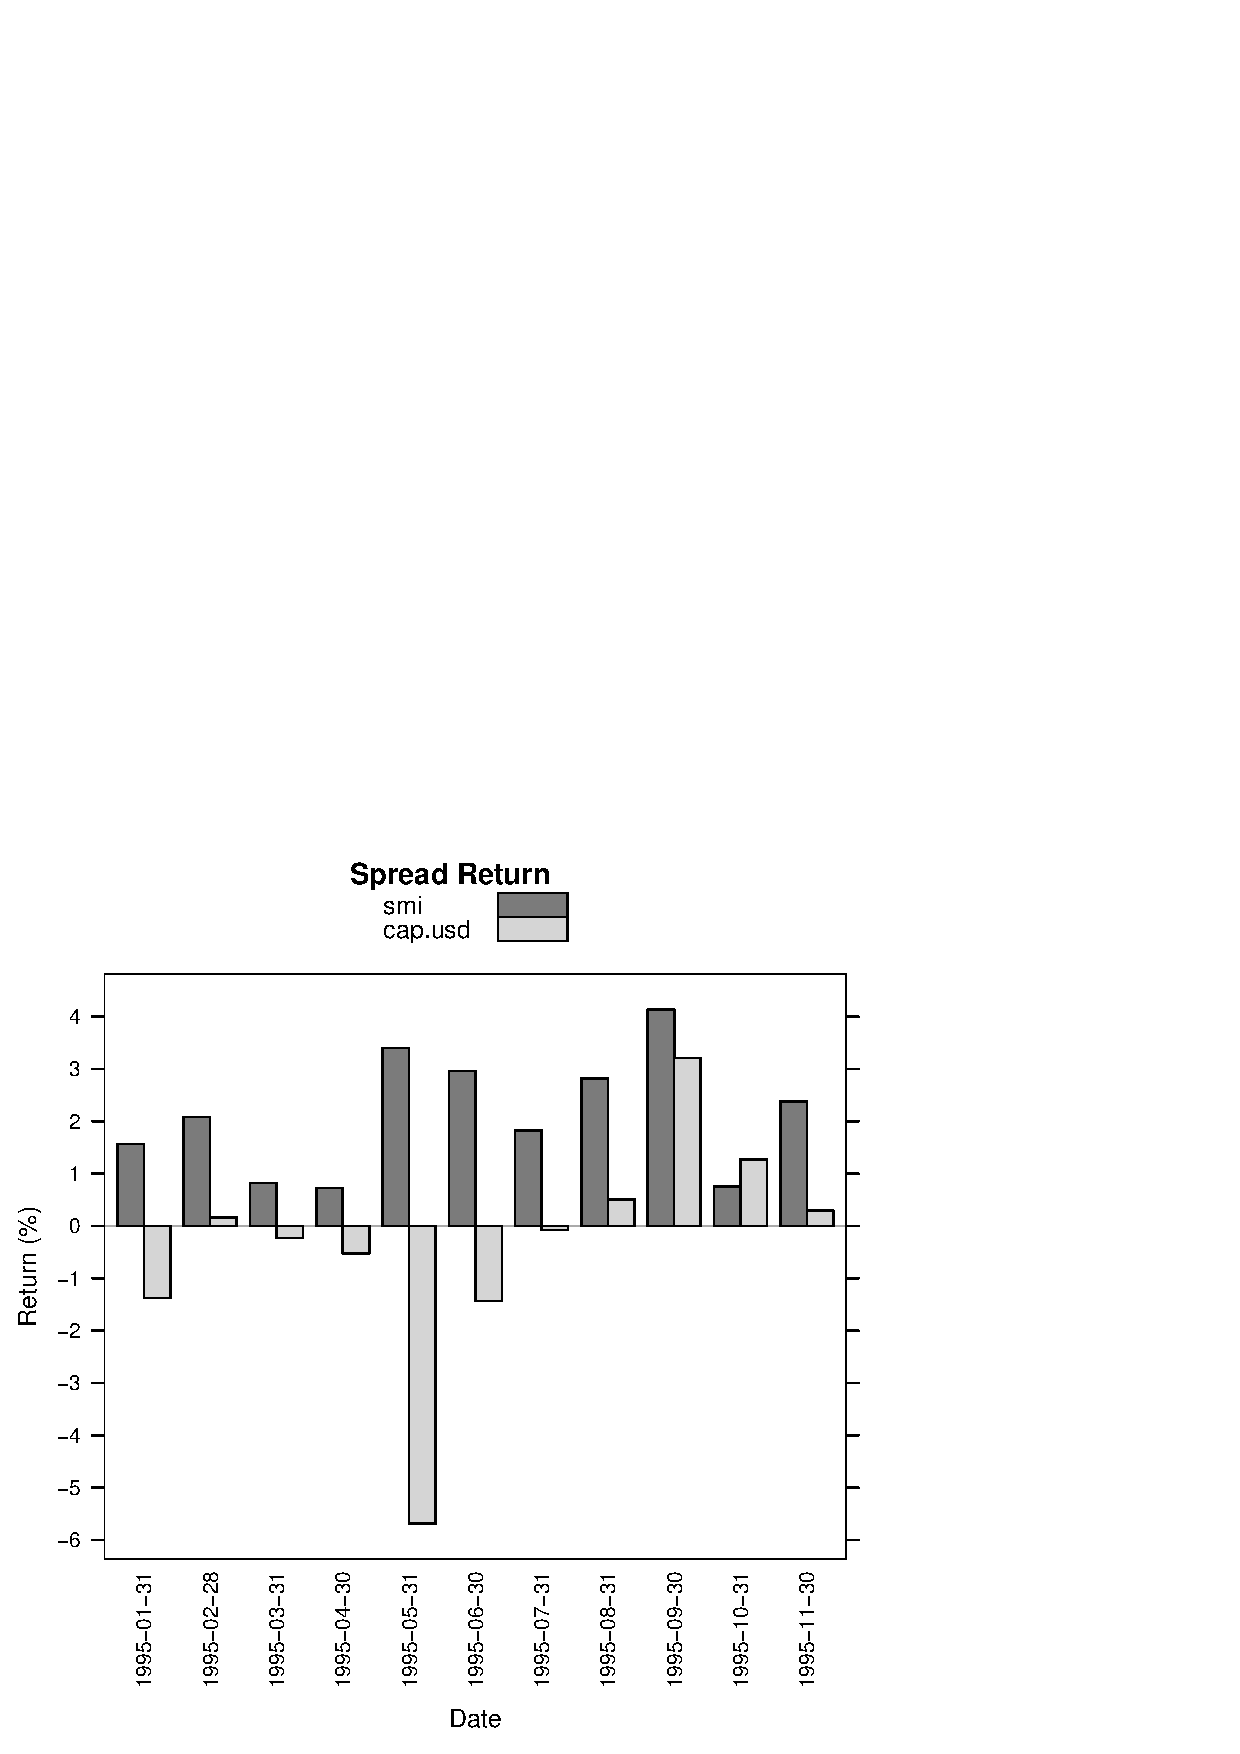
\includegraphics{backtest-020}
\caption{\label{figure:return}
Monthly return spreads.}
\end{figure}

Returns for \texttt{smi} were consistently positive.  Returns for
\texttt{cap.usd} were of low quality, but improved later in the
backtest period.  \texttt{cap.usd} had a particularly poor return in
June.

In addition to displaying the individual spread returns, we can also
visualise cumulative returns for each input variable:

\begin{figure}
\centering
\vspace*{.1in}
\begin{Schunk}
\begin{Sinput}
> plot(bt.save, type = "cumreturn.split")
\end{Sinput}
\end{Schunk}
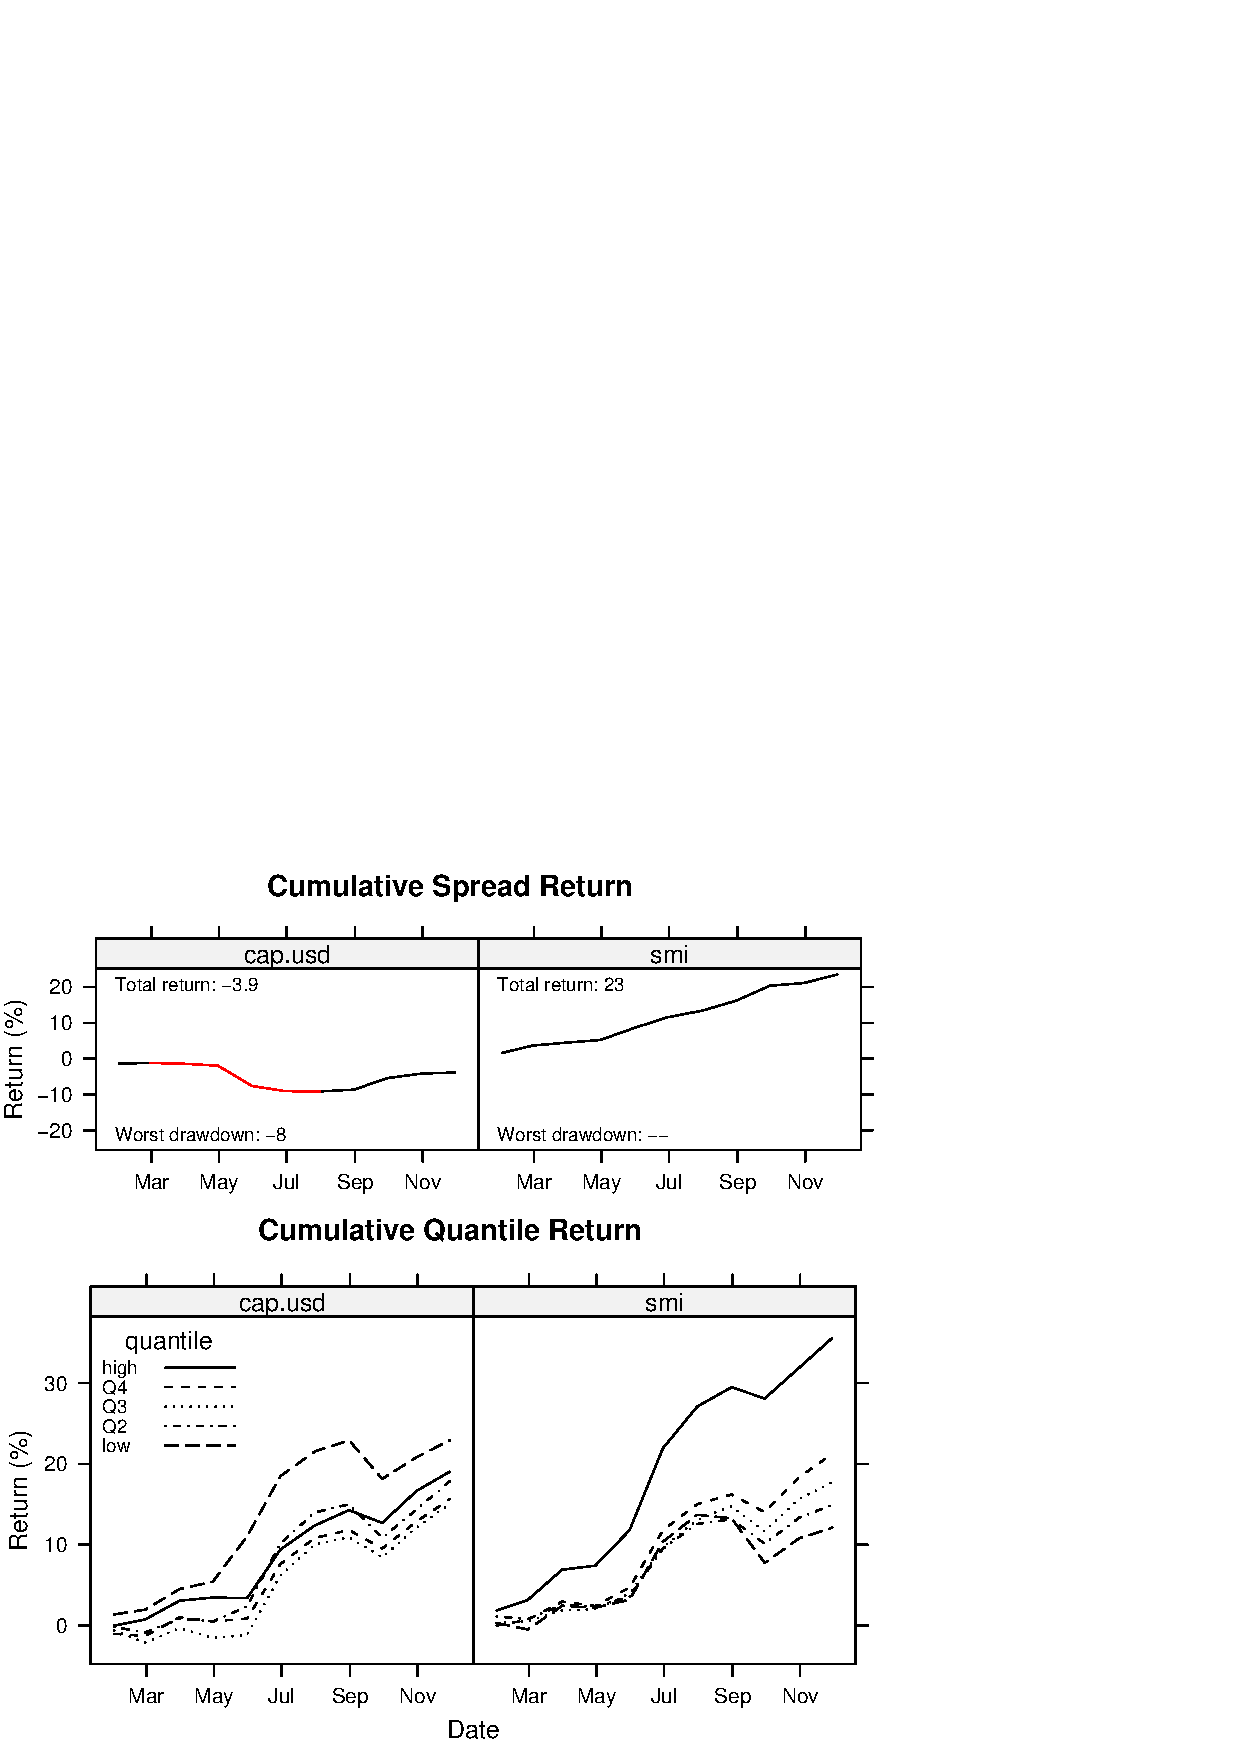
\includegraphics{backtest-021}
\caption{\label{figure:fanplot}
Cumulative spread and quantile returns.}
\end{figure}

The top region in this plot shows the cumulative return of each signal
on the same return scale, and displays the total return and worst
drawdown of the entire backtest period.  The bottom region shows the
cumulative return of the individual quantiles over time.  From this
chart we can see that \texttt{smi}'s top quantile performed best and
lowest quantile performed worst.  In contrast, \texttt{cap.usd}'s
lowest was its best performing quantile.

Though it is clear from the summary above that \texttt{smi} generated
about 5 times as much turnover as \texttt{cap.usd}, a plot is
available to show the month-by-month turnover of each signal:

\begin{figure}
\centering
\vspace*{.1in}
\begin{Schunk}
\begin{Sinput}
> plot(bt, type = "turnover")
\end{Sinput}
\end{Schunk}
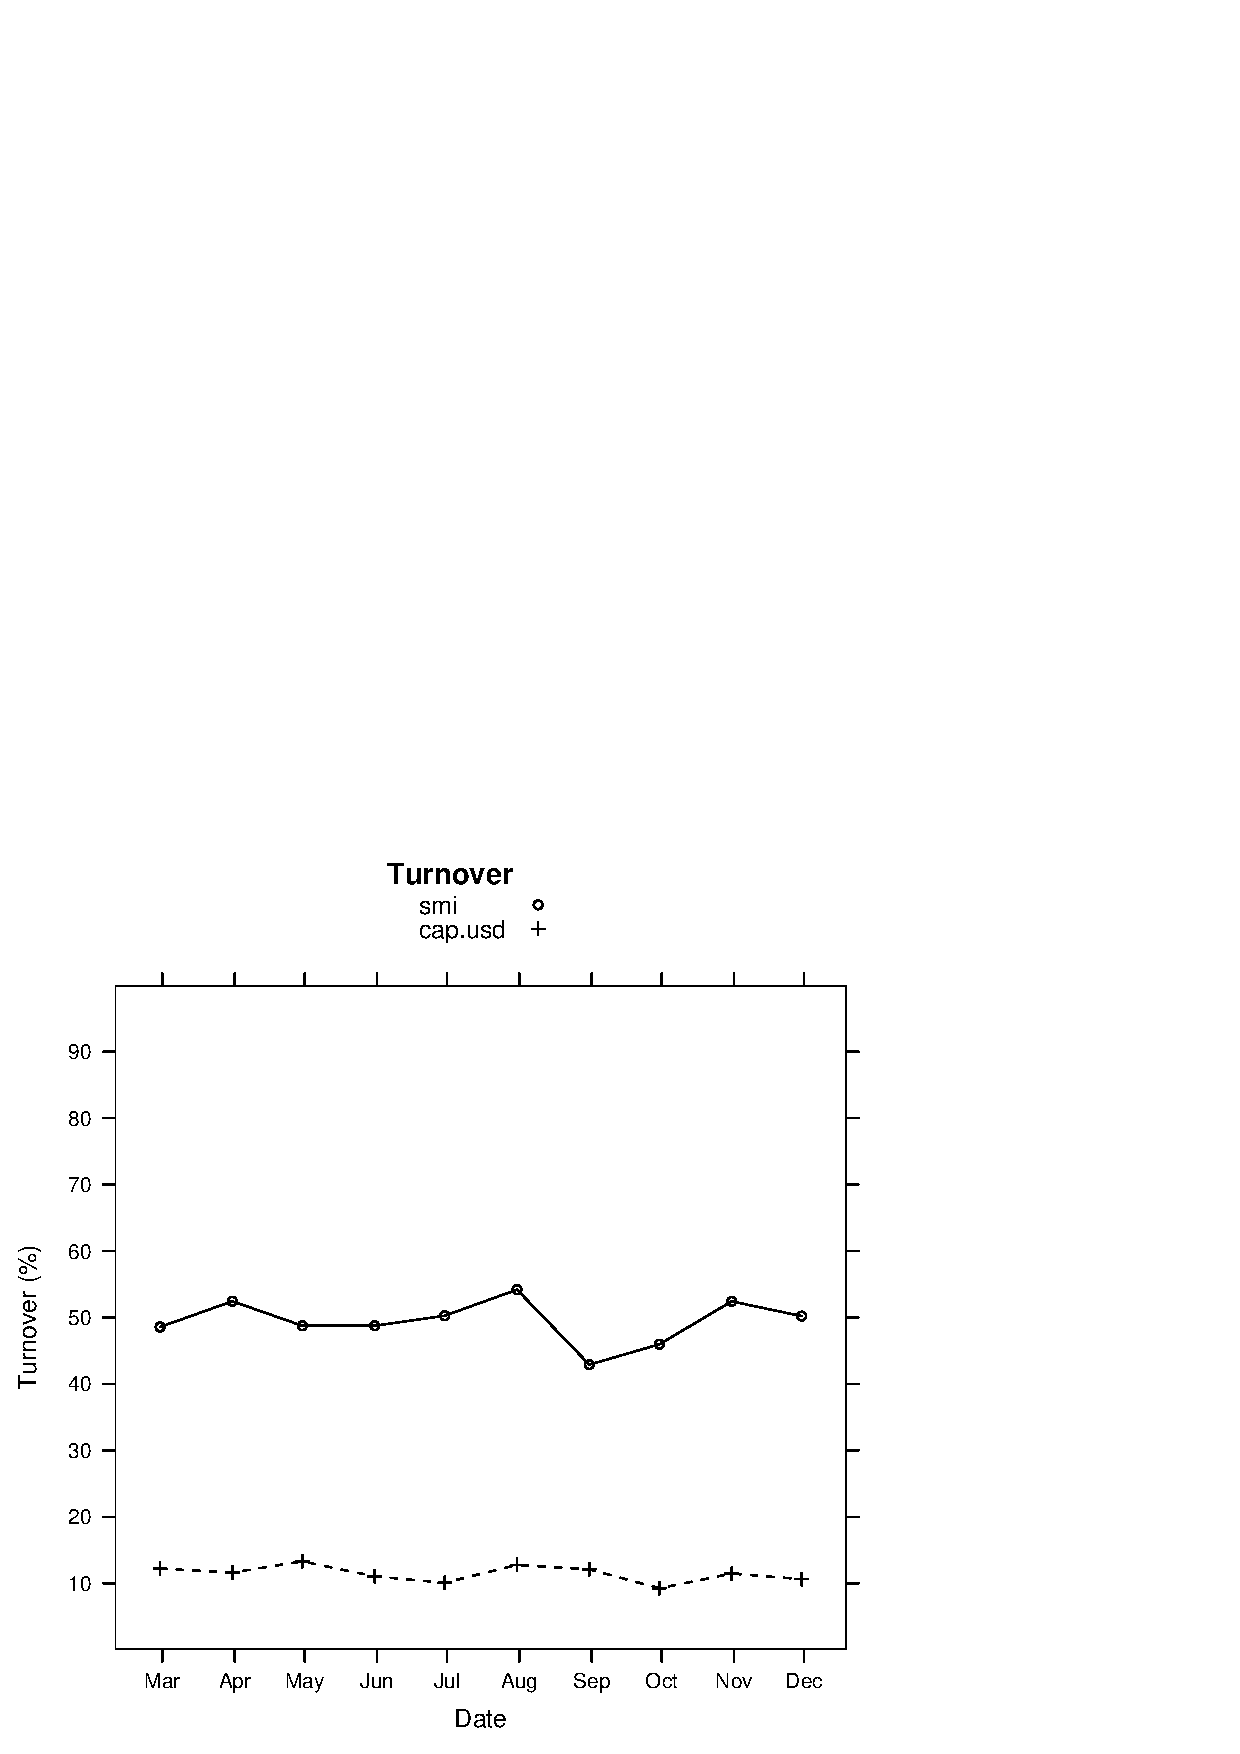
\includegraphics{backtest-022}
\caption{\label{figure:turnover}
Monthly turnover.}
\end{figure}

This chart shows that the turnover of \texttt{smi} was consistently
around 50\% with lower turnover in September and October, while the
turnover of \texttt{cap.usd} as an input signal was consistently
around 10\%.

\section*{Using \texttt{by.var}}

In another type of backtest we can look at quantile spread returns
\emph{by} another variable.  Specifying \texttt{by.var} breaks up
quantile returns into categories defined by the levels of the
\texttt{by.var} column in the main dataset.  Here we run a backtest
where we evaluate \texttt{smi} performance relative to one month
return by \texttt{sector}:


\begin{Schunk}
\begin{Sinput}
> bt <- backtest(starmine, in.var = "smi", 
+     ret.var = "fwd.ret.1m", by.var = "sector")
\end{Sinput}
\end{Schunk}


\begin{Schunk}
\begin{Sinput}
> summary(bt)
\end{Sinput}
\begin{Soutput}
Backtest conducted with:

1 in.var: smi;
1 ret.var: fwd.ret.1m;
and by.var: sector.

         low     2     3     4 high spread
Durbl 0.0063 0.007 0.009 0.007 0.01  0.004
Enrgy 0.0152 0.014 0.017 0.019 0.04  0.024
HiTec 0.0237 0.016 0.026 0.029 0.05  0.024
Hlth  0.0395 0.036 0.021 0.038 0.05  0.006
Manuf 0.0005 0.005 0.014 0.009 0.02  0.022
Money 0.0190 0.024 0.021 0.026 0.04  0.017
NoDur 0.0036 0.010 0.010 0.019 0.03  0.025
Other 0.0045 0.006 0.015 0.017 0.02  0.017
Shops 0.0020 0.004 0.005 0.017 0.03  0.026
Telcm 0.0277 0.014 0.022 0.023 0.03  0.005
Utils 0.0128 0.021 0.013 0.016 0.02  0.007
\end{Soutput}
\end{Schunk}


This backtest categorises observations by the quantiles of
\texttt{smi} and \texttt{sector}.  The highest spread return of 2.6\%
occurs in \texttt{Shops}.  Since \texttt{smi} quantiles were computed
before observations were split into groups by \texttt{sector},
however, we can not tell from this display roughly how much confidence
we should have in that return calculation.  There could be very few
observations in that sector or one of the top and bottom quantiles
could have a disproportionate number of observations, making the
return calculation suspect.  We can take a look by calling
\texttt{counts}:

\begin{Schunk}
\begin{Sinput}
> counts(bt)
\end{Sinput}
\begin{Soutput}
$smi
       low    2    3    4 high
Durbl  348  349  261  231  223
Enrgy  246  250  158  130   64
HiTec  647  660  824 1004 1432
Hlth   380  377  410  464  424
Manuf 1246 1265 1279 1395 1576
Money  959 1265 1244 1095  875
NoDur  615  563  528  441  371
Other 1034  940  784  760  710
Shops  870  714  710  697  548
Telcm  186  177  140  129   95
Utils  152  245  252  198  130
\end{Soutput}
\end{Schunk}

While there seems to be an adequate number of observations in
\texttt{Shops}, it is important to note that there are approximately
60\% more observations contributing to the mean return of the lowest
quantile than to the mean return of the highest quantile.  Overall, we
should be more confident in results for \texttt{Manuf} and
\texttt{Money} due to their consistently high counts across quantiles.
We might want to examine the result for \texttt{HiTec} more closely,
however, since there are more than twice the number of observations in
the highest quantile than the lowest.

\texttt{by.var} can also be numeric, as in this backtest using
\texttt{cap.usd}:


\begin{Schunk}
\begin{Sinput}
> bt <- backtest(starmine, 
+     in.var = "smi", ret.var = "fwd.ret.1m", 
+     by.var = "cap.usd", 
+     buckets = c(5, 10))
\end{Sinput}
\end{Schunk}


\begin{Schunk}
\begin{Sinput}
> summary(bt)
\end{Sinput}
\begin{Soutput}
Backtest conducted with:

1 in.var: smi;
1 ret.var: fwd.ret.1m;
and by.var: cap.usd.

        low      2      3     4  high spread
low  0.0105 0.0139 0.0236 0.028 0.038  0.028
2    0.0078 0.0093 0.0216 0.025 0.046  0.038
3    0.0186 0.0072 0.0167 0.031 0.034  0.016
4    0.0124 0.0142 0.0139 0.013 0.038  0.026
5    0.0080 0.0124 0.0087 0.010 0.025  0.017
6    0.0126 0.0121 0.0191 0.021 0.026  0.013
7    0.0080 0.0070 0.0160 0.019 0.034  0.026
8    0.0050 0.0181 0.0101 0.014 0.027  0.022
9    0.0104 0.0153 0.0167 0.014 0.028  0.018
high 0.0156 0.0207 0.0133 0.023 0.026  0.011
\end{Soutput}
\end{Schunk}

Since \texttt{cap.usd} is numeric, our obervations are now split by
two sets of quantiles.  The quantiles listed aross the top are, as
before, the input variable quantiles of \texttt{smi}.  Down the side
are the quantiles of \texttt{cap.usd}.  We controlled the number of
quantiles by using the \texttt{buckets} parameter of
\texttt{backtest}. The higher returns in the lower quantiles of
\texttt{cap.usd} suggests that \texttt{smi} might perform better in
small cap stocks than in large cap stocks.

\section*{Multiple return horizons}

Using \texttt{backtest} we can also analyse the performance of a
signal relative to multiple return horizons.  Below is a backtest that
considers one month and six month forward returns together:

%\DefineVerbatimEnvironment{Soutput}{Verbatim}{fontsize=\scriptsize}
%\DefineVerbatimEnvironment{Sinput}{Verbatim}{fontsize=\footnotesize}

\begin{Schunk}
\begin{Sinput}
> bt <- backtest(starmine, in.var = "smi", 
+     buckets = 4, ret.var = c("fwd.ret.1m", 
+         "fwd.ret.6m"))
\end{Sinput}
\end{Schunk}


\begin{Schunk}
\begin{Sinput}
> summary(bt)
\end{Sinput}
\begin{Soutput}
Backtest conducted with:

1 in.var: smi;
2 ret.vars: fwd.ret.1m, fwd.ret.6m;
and no by.var.

             low     2     3 high spread
fwd.ret.1m 0.011 0.015 0.018 0.03  0.019
fwd.ret.6m 0.112 0.121 0.142 0.17  0.059
\end{Soutput}
\end{Schunk}


%\DefineVerbatimEnvironment{Sinput}{Verbatim}{fontsize=\small}
%\DefineVerbatimEnvironment{Soutput}{Verbatim}{fontsize=\small}

The performance of \texttt{smi} over these two return horizons tells
us that the power of the signal degrades after the first month.  Using
six month forward return, \texttt{fwd.ret.6m}, the spread is 6\%.
This is only 3 times larger than the 2\% spread return in the first
month despite covering a period which is 6 times longer. In other
words, the model produces 2\% spread returns in the first month but
only 4\% in the 5 months which follow.


\section*{Conclusion}

The \pkg{backtest} package provides a simple yet powerful collection
of tools for performing portfolio-based tests of financial hypotheses
by making a set of simplifying assumptions.  A much more complex
package, \pkg{portfolioSim}, provides facilities for historical
portfolio performance analysis outside these assumptions.  Built on
the framework of the \pkg{portfolio}\footnote{See \cite{kane:david}
  for an introduction to the \pkg{portfolio} package.} package,
\pkg{portfolioSim} tackles the issues of exposure and liqudity
constraints, as well as arbitrary portfolio construction and trading
rules.  Before reaching that level of complexity, however,
\pkg{backtest} provides a good starting point for testing a new
hypothesis.

  \address{Kyle Campbell, Jeff Enos, Daniel Gerlanc and David Kane \\
    Kane Capital Management \\
    Cambridge, Massachusetts, USA\\
    \email{Kyle.W.Campbell@williams.edu}, \email{jeff@kanecap.com},
    \email{dgerlanc@gmail.com} and \email{david@kanecap.com}}

\bibliography{backtest}

\end{article}
\end{document}
